\documentclass[10pt,foldmark,tumble]{leaflet}
\usepackage[utf8]{inputenc}
\usepackage{mathptmx}
\usepackage{url}
\usepackage{graphicx,txfonts}
\usepackage[dvipsnames,usenames]{color}

\newcommand{\love}{\ensuremath\varheartsuit\ }

\CutLine*{1}% Dotted line without scissors
\CutLine*{6}
%%\CutLine{6}%  Dotted line with scissors

\AddToBackground{1}{%  Background of a small page
  \put(200,560){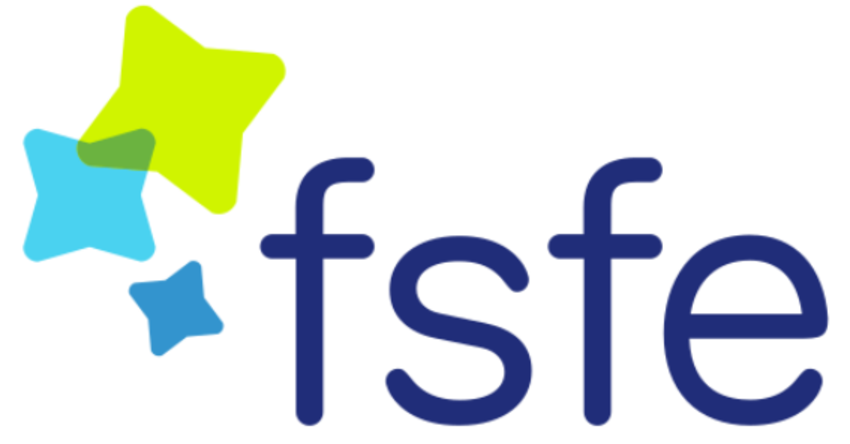
\includegraphics[scale=0.14]{logo.pdf}}}


%%\AddToBackground{6}{%  Background of a small page
%%  \put(0,0){\textcolor{Cyan}{\rule{\paperwidth}{\paperheight}}}}


\begin{document}

\section{
\includegraphics{item.png}Acerca de}

La Fundación del Software Libre de Europa es una organización benéfica que faculta a los usuarios para controlar la tecnología.

El software está muy involucrado en todos los aspectos de nuestras vidas; y es importante que esta tecnología nos confiera poder en lugar de restringirnos. El Software Libre otorga a todo el mundo el derecho a usar, entender, adaptar y compartir software. Estos derechos ayudan a apoyar otras libertades fundamentales como la libertad de expresión, de prensa y la privacidad.

\section{
\includegraphics{item.png}Nuestro Trabajo}

 Mediante su caracter como organización no gubernamental, la Fundación europea del Software Libre (Free Software Foundation Europe, en inglés) trabaja en pos de un mejor conocimiento y respaldo del Software Libre y los Estándares Abiertos en el ámbito político, económico, legal y en definitiva, en toda nuestra sociedad.

 \subsection{Legal}

    A través de nuestro equipo legal, recogemos y compartimos información y conocimientos sobre aspectos legales y de licencias de Software Libre, salvaguardamos el interés de los proyectos de Software Libre, conectamos expertos en todo el mundo y ayudamos a otros grupos en su actividad para lograr fines similares. Proveemos asistencia, formación y documentación, en estrecha colaboración con \url{gpl-violations.org} y los miembros de la European Legal Network (Red Jurídica Europea).
        
\subsection{Sensibilización ciudadana}

    Informar a nuestra sociedad sobre el Software Ligre es una de las misiones principales de FSFE. Contamos con expertos en muchos de los temas y asuntos relacionados con el Free Software y que pueden ser contactados para ofrecer conferencias, organizar talleres y worksihps o para participar en debates.
    
\subsection{Estándares Abiertos}

    Los Estándares Abiertos (Open Standards en inglés) permiten la distribución e intercambio de todo tipo de datos de una forma libre y con total precisión. Previenen "lock-in (dependencia tecnológica) y otras barreras artificiales que impiden la interoperabilidad. Además, promocionan la oferta entre comerciantes y soluciones tecnológicas. El trabajo de FSFE en relación a los Estándares biertos busca asegurar la facilidad de migración entre Free Software o entre sus diferences soluciones.
    
\subsection{Patentes de Software en Europa}

    Las patentes de Software son una amenaza para la sociedad y la economía. Restringuen la innovación, dañan la economía y amenazan la creatividad colaborativa. FSFE lucha por una Europa libre de patentes de sfotware y trabaja en el nivel internacional, en el ámbito de las Naciones Unidas, para erradicar las patentes de software a nivel mundial.

\subsection{Unión Europea}

    FSFE trabaja en la Comisión Europea y el Parlamento Europeo para crear un entorno pro Software Libre y Estándares Abiertos en Europa. Luchamos contra los monopolios y por un mercado de software competitivo participando como tercera parte en casos antimonopolio. Informamos a la clase política sobre las diversas oportunidades que el Software Libre ofrece y apostamos por la interoperabilidad.

\subsection{Educación}

    FSFE promociona activamente el uso de Software Libre en colegios y universidades. El Software Libre es pedagógicamente superior, su espíritu básico implica tanto libertad como cooperación, dos factores educativos básicos para consolidar la democracia.
    
\subsection{Naciones Unidas}

    FSFE ha estado presente en Naciones Unidas desde 2002, ayudando a crear una sociedad de la información global más libre y justa. Actualmente, estamos trabajando activamente en las siguientes áreas:
    
    \begin{itemize}
    \item World Intellectual Property Organization(Organización Mundial de la Propiedad Intelectual)
    \item Internet Governance Forum(Foro de la Gobernabilidad de Internet)
    \end{itemize}

\section{
\includegraphics{item.png}Campañas}

Como ONG sin ánimo de lucro, la FSF Europa trabaja para soportar y dar a conocer el Software Libre y los Estándares Abiertos en la política, los negocios, las leyes y la sociedad en su conjunto. Por eso lanzamos las siguientes campañas. ¡Puedes ayudarnos con ellas!

\subsection{Secure Boot}

    El objetivo de la FSFE es asegurar que los propietarios de dispositivos tecnológicos mantengan el control total y único de ellos. Este principio fundamental ha sido desafiado recientemente.

\subsection{PDFreaders.org}

    Lanzado por la Fellowship of FSFE, pdfreaders.org es un sitio que provee información sobre lectores PDF de Sotware Libre para todos los sistemas operativos mayoritarios.
    
\subsection{Document Freedom Day}

    Cada año, el DFD es el día para aumentar la conciencia sobre los Formatos Abiertos de Documento (ODF) y los Estándares Abiertos organizando actividades por todo el mundo junto con organizaciones asociadas y voluntarios.

\subsection{Hacia una World Intellectual Wealth Organization}

    Respaldamos y soportamos la Declaración de Ginebra, e invitamos a sus redactores, signatarios, y a las Naciones Unidas a empezar a pensar no sólo cuál debería ser el rol de la WIPO, sino en qué tipo de organización debería convertirse en el futuro para gestionar nuestra riqueza intelectual.

\subsection{Pregunta a tus candidatos}

    Durante elecciones locales, federales y parlamentarias, la FSFE hace una llamada a todos los defesores del Software Libre para preguntar a los partidos sus posiciones respecto el Softyware Libre y los Estándares Abiertos.

\subsection{I \love Software Libre}

    El Día de San Valentín es una celebración de amor y afecto entre compañeros íntimos. La campaña de la FSFE intenta crear la oportunidad de mostrar que te importan la gente y el Software Libre a los que amas durante todo el año.
    
\subsection{¡Libera Tu Android!}

    Android es un sistema operativo en su mayor parte libre desarrollado principalmente por Google. Por desgracia, los controladores para la mayoría de dispositivos y la mayoría de aplicaciones no son libres. Esta campaña recolecta información sobre correr un sistema Android lo más libre posible e intenta coordinar estos esfuerzos.
    
\subsection{DRM.info}

    DRM.info es una plataforma colaborativa iniciada y mantenida por la FSFE para informar sobre los peligros de la Gestión Digital de Restricciones (DRM) y hacer visible la preocupación de varios grupos diversos. Los contribuyentes de DRM.info incluyen grupos de libertad digital, organizaciones de protección al consumidor, net-activismo y bibliotecas.
    
\subsection{EURA v. las Autoridades Tributarias Eslovacas}

    EURA es un caso pendiente de litigio estratégico para los Estándares Abiertos en Eslovaquia. En 2010, Eslovaquia ordenó utilizar medios electrónicos como única forma de completar ciertas obligaciones tributarias. Sin embargo, la solución electrónica del estado estuvo disponible sólo para clientes de un proveedor. EURA, un importador textil eslovaco, fue multado por no usar este proveedor.

\section{
\includegraphics{item.png}Colabore}

 Somos una comunidad de personas que se comprometen con el Software Libre. ¡Por favor, únase y trabaje con nosotros! Hay muchas maneras de hacerlo, seguro que encuentra una que encaje con sus intereses y habilidades.

\subsection{Corra la voz}

    Reparta folletos, pegatinas o carteles a sus amigos, colegas o distribúyalos en público, y use nuestras imágenes optimizadas para la web.
    
\subsection{Participe en nuestras discusiones}

    La mayor parte de nuestro trabajo se coordina mediante listas de correo. Participe en las discusiones, aprenda de otros, y moldee las posturas de la FSFE.

\subsection{Reúnase con nosotros}

    Si quiere reunirse con nosotros, venga a un evento que tenga lugar cerca de usted, inclyendo charlas, puestos de información o encuentros de grupos locales de Fellowship.
    
\subsection{Mejore nuestra web}

    Para muchas personas nuestra web es la primera impresión que obtienen de nosotros. Como webmaster puede determinar la eficacia de nuestra comunicación con el mundo.
    
\subsection{Ayude como diseñador}

    La FSFE y la comunidad del Software Libre necesitan a menudo diseñadores para el material electrónico e impreso. Únase a nuestro equipo y vea sus diseños diseminados por todo el mundo.
    
\subsection{Prácticas para becarios}

    Aprenda a trabajar en una organización paneuropea que opera en un entorno internacional. A la vez que trabajamos por la libertad del software, tratamos asuntos sociales, politicos y legales cada día, y usted también podrá hacerlo.

\subsection{Traduzca y revise}

    Algunas páginas de nuestra web están disponibles en más de 30 idiomas pero otras todavía no lo están. Ayúdenos a llegar al mayor número de personas posible traduciendo nuestros artículos, notas de prensa y boletines de noticias a un idioma que conozca.
    
\subsection{Conviértase en un miembro que apoya económicamente}

    Las donaciones son críticas para nuestra fuerza y autonomía. Conviértase en un miembro sostenedor uniéndose a la Fellowship y permitiéndonos continuar la lucha por el software libre donde sea necesaria.
    
\vspace{15em}


\centering 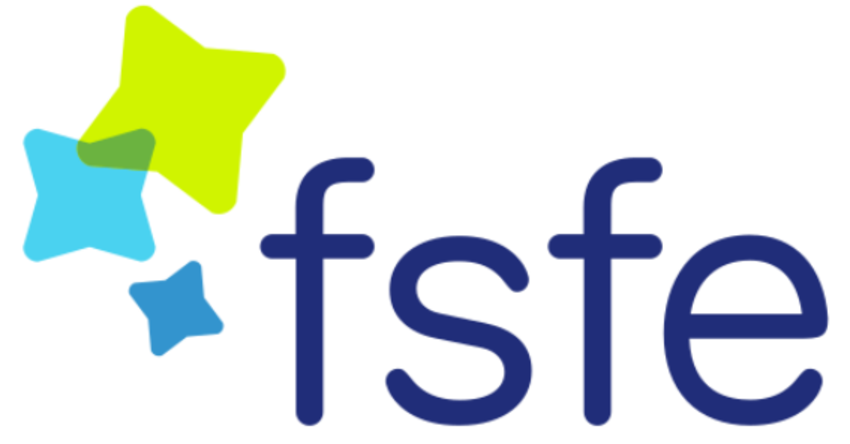
\includegraphics[scale=0.45]{logo.pdf} \\
\centering \Huge \url{fsfe.org}


\end{document}
